\epigraph{Wenn die Natur deterministisch ist, könnte ein Quantencomputer mehr sein als ein Wahrscheinlichkeitsrechner.}{}

\section{Deterministische Quantenlogik}


\begin{figure}[htbp]
\centering
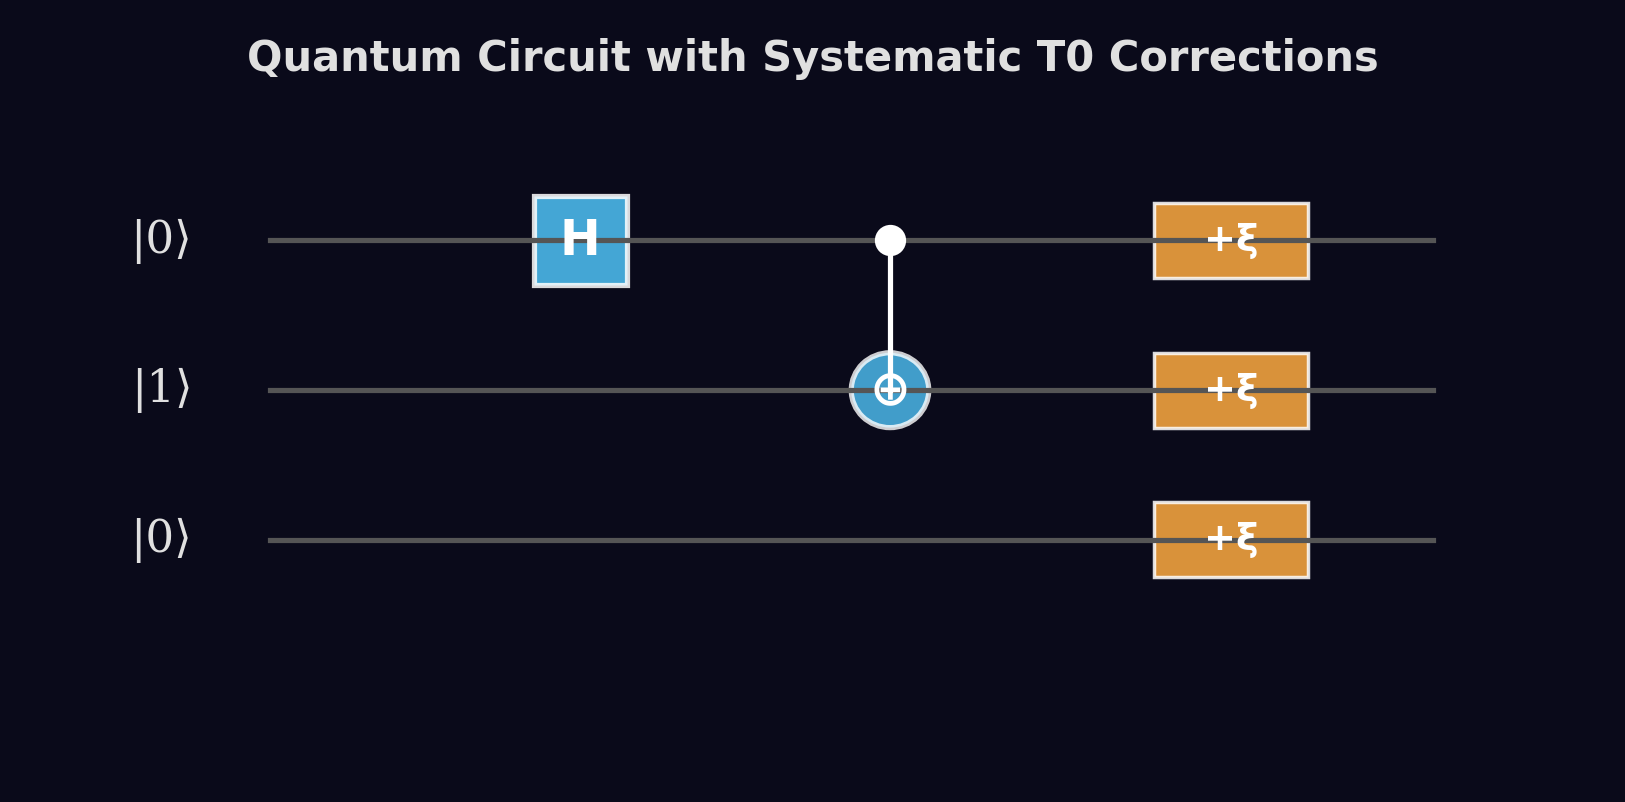
\includegraphics[width=0.85\textwidth]{img/ch10_quantum_circuit.png}
\caption{Quantenschaltkreis mit systematischen $\xi$-Korrekturen an jedem Gatter.}
\end{figure}
Die Standardinterpretation der Quantenmechanik sagt: Quantenzufall ist fundamental. T0 sagt etwas anderes: \emph{Quantenzufall ist eine Illusion deterministischer Zeitfeld-Dynamik.} Die Konsequenzen für Quantencomputer sind erheblich.

\section{T0-Qubits}

In der T0-Beschreibung sind Qubits keine probabilistischen Zustände, sondern Energiefeld-Konfigurationen:
\begin{align}
|0\rangle_{\text{T0}} &\leftrightarrow \delta E_0(x,t) = E_0 \cdot f_0(x,t) \\
|1\rangle_{\text{T0}} &\leftrightarrow \delta E_1(x,t) = E_1 \cdot f_1(x,t)
\end{align}

Die Basiszustände sind nicht \enquote{gleichzeitig vorhanden} im Sinne einer echten Superposition. Sie sind verschiedene Konfigurationen des Vakuumfeldes, deren deterministische Evolution so komplex ist, dass sie \emph{praktisch} nur probabilistisch beschrieben werden kann.

\section{Modifizierte Quantengatter}

Die T0-Korrekturen an Quantengattern sind klein, aber messbar. Das Hadamard-Gatter erhält eine $\xsi$-Korrektur:
\begin{equation}
H_{\text{T0}} = H \cdot \left(1 + \xsi \cdot \frac{\langle \delta E \rangle}{E_{\text{Planck}}}\right)
\end{equation}

Der Shor-Algorithmus zur Faktorisierung verbessert sich leicht: $P_{\text{Erfolg}}^{\text{T0}} = P_{\text{Standard}} \cdot (1 + \xsi\sqrt{n})$. Der Grover-Algorithmus zur Suche benötigt weniger Iterationen: $N_{\text{Iter}}^{\text{T0}} = (\pi/4)\sqrt{N} \cdot (1 - \xsi \cdot \ln N)$.

\section{Dekohärenz-Unterdrückung und Bell-Korrekturen}

Besonders vielversprechend ist die fraktale $\xsi$-Dämpfung, die eine natürliche Stabilisierung gegen Dekohärenz bietet. Und die T0-Korrekturen an den Bell-Ungleichungen --- CHSH-Abweichungen der Größenordnung~$10^{-3}$ in 73-Qubit-Systemen --- sind mit heutiger Technologie experimentell testbar.

Zwei fundamentale Probleme der Quantenmechanik lösen sich in T0 auf: Das Messproblem verschwindet, weil es keinen Wellenfunktionskollaps gibt --- nur kontinuierliche Zeitfeld-Evolution. Und die \enquote{spukhafte Fernwirkung} der Verschränkung wird zur lokalen Korrelation durch gemeinsame Zeitfeld-Geschichte (vgl.\ \href{https://github.com/jpascher/T0-Time-Mass-Duality/blob/main/2/pdf/020_T0_QM-QFT-RT_De.pdf}{Dok.~020}, \href{https://github.com/jpascher/T0-Time-Mass-Duality/blob/main/2/pdf/131_scheinbar_instantan_De.pdf}{131}, \href{https://github.com/jpascher/T0-Time-Mass-Duality/blob/main/2/pdf/147_quantum_computing_De.pdf}{147} für die vollständigen Herleitungen).

\begin{kerngedanke}
Die T0-Korrekturen an Quantencomputern sind klein, aber systematisch. Sie bieten keine Revolution der Quanteninformatik, aber etwas möglicherweise Wichtigeres: testbare Vorhersagen, die zwischen der Standardinterpretation und T0 unterscheiden können.
\end{kerngedanke}
